

\chapter{Geographical data}

\pagestyle{fancy}

From all GIS subsystems, the data one is probably the most important one. It is also the more interrelated, as it is linked to all of them and all depend on it to a certain extent. Data is the fuel that drives GIS. 

\section{Data and information. Types of information.}

There is a big difference between the concepts of \textbf{data} and \textbf{information}. A GIS is a Geographical \emph{Information} System, but it uses geographical \emph{data}.

Data is a \textbf{set of values of elements used to represent something}. For instance, the string 502132N is a data.

We can interpret that data as being a geographical reference, in which case it could be a latitude value, in particular 50\degree $21'$ $32''$ North. If we interpret it as being a reference to an identity card (such as a driver's license) associated with a person, the information that we get is completely different. It is the same data, containing six digits and a letter, but the information that we extract from it is different, since we understand and interpret it differently. 

Information is, therefore, the result of data and \textbf{its interpretation}. and in many cases, working with data means just trying to extract from it all the information that it might contain.

Understanding the meaning and the differences between data an information allows us to understand, for instance, why the ratio between the size of a given data and the amount of information it contains is not constant. The strings 502132NORTH and FIFTY TWENTY ONE THIRTY TWO NORTH are longer than 502132N, but they contain the same information (as long as we interpret them as the latitude component of a coordinate).

Geographical information has two separate components: \textbf{spatial} and \textbf{thematic}. The spatial component contains the position, referred to a given reference system, and it answers the question \emph{where?}. The thematic component answers the question \emph{what?}, and it defines the characteristics of the phenomenon or feature that occurs at the location indicated by the spatial component.

While the spatial component is usually a numerical value (most coordinate systems use just numbers), the thematic component can be \textbf{numeric} or \textbf{alphanumeric}. A numeric variable can be itself of four different types: \textbf{nominal, ordinal, interval} or \textbf{ratio}.

The operations that can be performed on a certain geographical data are defined by the types of variables contained in its thematic component.

The different approaches for representing and storing geographical information, which we will see later in this same chapter, depend on the type of variable that we are working with.

An important concept to consider related to geographical information is the \textbf{dimension}. The elements that we store range from simple points (0D), to three-dimensional volumes (3D) (Figure \ref{Fig:Dimensions}).

\begin{figure}[!hbt] 
\centering
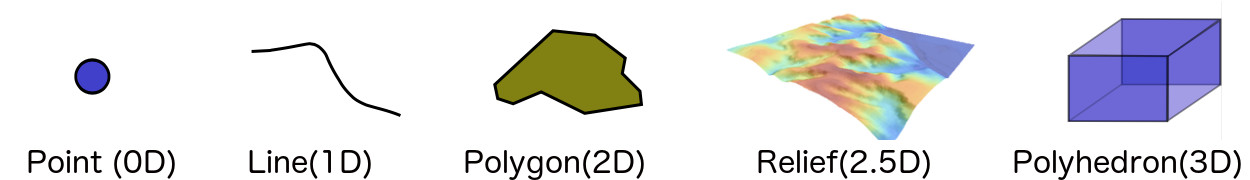
\includegraphics[width=\textwidth]{Data/Dimensions.png}
\caption{\small Dimensions of the spatial component of geographical data.}
\label{Fig:Dimensions} 
\end{figure}


\section{Subdivision of information. Layers}

In a GIS, the information about a given study area \textbf{is divided in several levels}. Even if it refers to the same location, the information about different variables is stored separately. That is, a set of different blocks of information exists for the same area, each of them containing a particular variable or set of elements. Each of these blocks is called a \textbf{layer}.(Figure \ref{Fig:Concept_layer}). 

\begin{figure}[!hbt] 
\centering
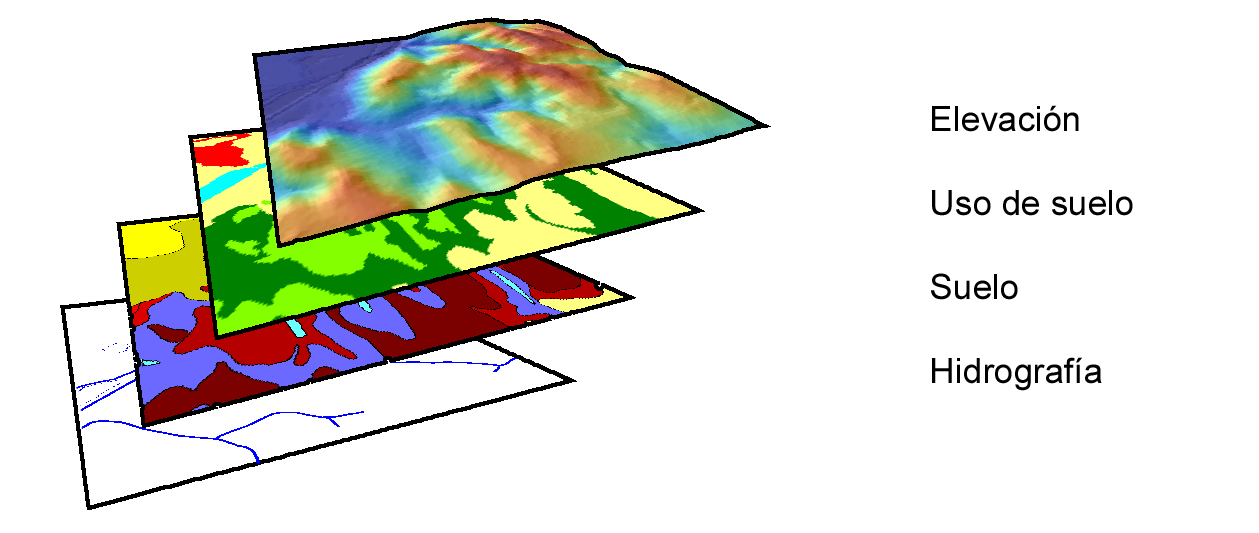
\includegraphics[width=\textwidth]{Data/Concept_layer.png}
\caption{\small A graphical explanation of the concept of \emph{layer}.}
\label{Fig:Concept_layer} 
\end{figure}

The concept of layer is fundamental to understand GIS, and it helps to correctly structure and manage geographical information. All the information that we will use in a GIS will be in the form of layers. Each one of them can be used independently or along with others.

With traditional cartography, it is not possible (or it is complex and not accurate) to combine different types of information, such as, for instance, the one contained in a topographic map and the one from a land-use map. In the case of a GIS, the different layers in which that information is contained can be combined in an easy and clean way.

The concept of layer as the fundamental unit for geographical information in GIS has a huge relevance, as it constitutes the basic framework for most operations. For instance, we saw in the section about cartographic generalization how in a GIS we can use different ``versions'' of the data corresponding to a given area, and show one or another depending on the current scale. This versions will be stored as independent layers. Layers are, thus, not just the fundamental unit for a given area, but also for a given scale, and allow to optimally separate and organize geographical information. 

Layers also help avoiding data redundancy, since each layer just contains information about a particular variable or type of feature. A traditional map always contains a set of different variables, not just a single one. Some of them are used to provide a general context, such as the names of the main cities or the main roads, and these appear in most maps. In a GIS, they exist independently, and the user can add them and combine them with other layers whenever is needed. Therefore, working with layers provides a more efficient approach and a \textbf{more atomized} organization of the data, with the advantages that it has for its storage, management and use.

Apart from dividing geographical information in layers depending on its content, it is also divided considering purely spatial criteria, ``cutting'' it in smaller parts that cover a smaller area. This is similar to what happens with traditional cartography, divided in \textbf{map sheets}.

The main feature of a GIS to transparently integrate data corresponding to different areas and create a seamless mosaic is the \textbf{separation between the data and its visualization}. Data is required for visualization, but these two elements constitute different parts of a GIS, with a clear separation between them. That means that data is used to create a visual output, but data itself does not contain any value related to its rendering and visualization.

Thus, it is possible to combine data and then represent that combination together as a whole. Something like that is not possible with a printed map, since it contain also the visualization elements (colors, line thickness, label placements, etc.) and even some additional cartographic ones (legend, scale, North arrow, etc.). Even if printed maps can be combined, information contained in them does not ``fuse'' to create a single new map. In a GIS, on the other hand, visualization of several blocks of data can be identical to the one that would be obtained if that data were stored as a single block.


\section{Geographical information models}

The process of converting a given geographical area and the information about it in a data that can be used within a GIS can be divided in three different phases.

\begin{itemize}
 \item Establishing a \textbf{geographical model}. That is, a conceptual model of a reality and its behavior.
\item Establishing a \textbf{representation model}. That is, a way of coding the conceptual model, reducing it to a finite set of elements.
\item Establishing a \textbf{storage model}. That is, a storage strategy for storing the elements of the representation model.
\end{itemize}

Representation models are the most important ones, and we will focus on them here. The two main representation models are the \textbf{raster model} and the \textbf{vector model}. Layers using these models are commonly known as \textbf{raster layers} and \textbf{vector layers}.

\subsection{Raster model}

The raster model is based on a \textbf{systematic division of space}. The whole space is characterized by a set of elements that cover it, each of them with an associated value.

The most common raster model is based on a grid of \textbf{square cells}, or sometimes rectangular ones. Knowing the orientation of the grid, the size of  the cells (which is the same for all of them), and at least the coordinates of one of them, it is possible to know the location of all cells, thanks to its \textbf{regular structure}. With that, the values of the variable we are working with are known in all points of the area that is covered by the layer. The \textbf{cell size} is a parameter related to the scale of the layer, since it defines its resolution and depends on the level of detail used when the corresponding measures were taken.

Figure \ref{Fig:Raster_closeup} shows an example of a raster grid.

\begin{figure}[!hbt]   
\centering
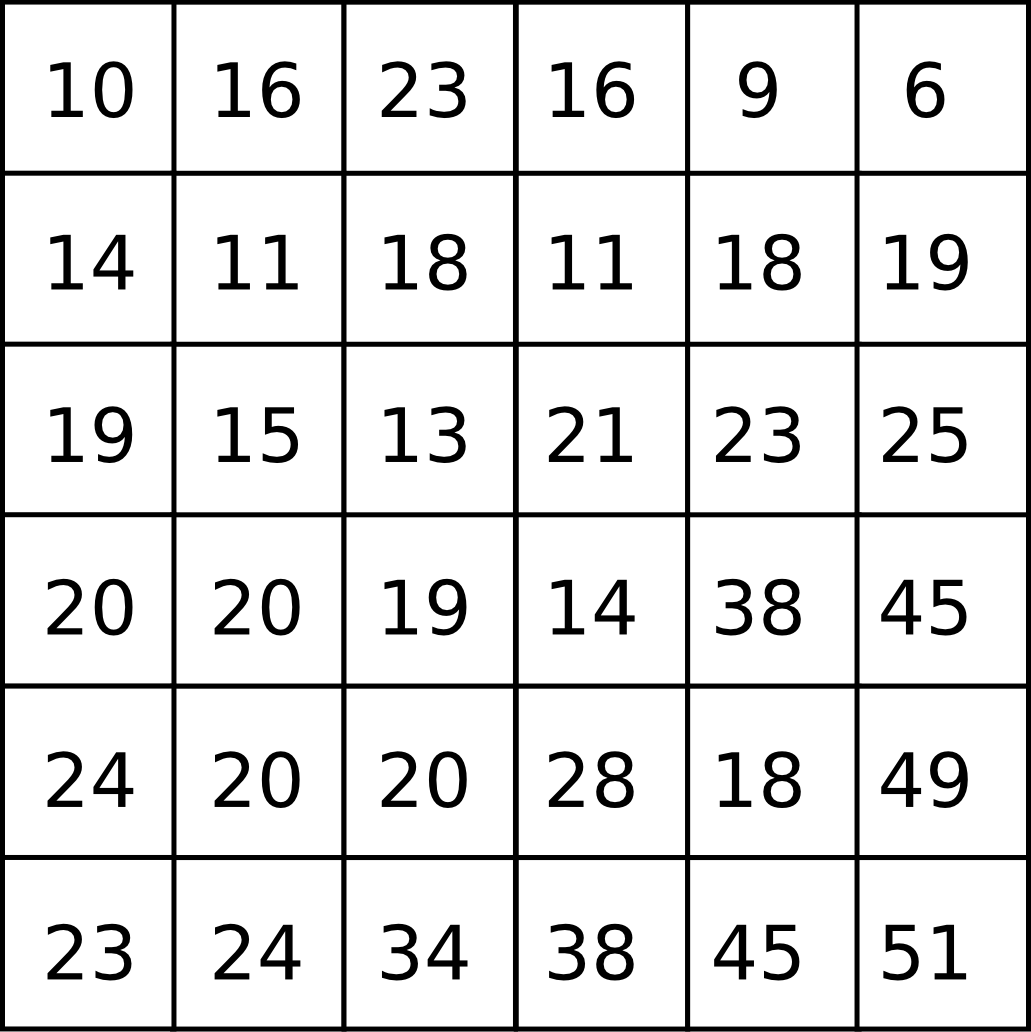
\includegraphics[width=.4\textwidth]{Data/Raster_closeup.png}
\caption{\small Cells in a raster grid with their associated values.}
\label{Fig:Raster_closeup} 
\end{figure}

The number of values stored for each cell defines the number of \textbf{bands} in a raster layer. A band contains a single value for each cell. We can understand a raster layer with more than one band as a set of sublayers, all of them having the same spatial structure (extent and cell size), and wrapped as a single layer.

We can find a clear example of that in digital color images. A digital image is composed of a grid of values (called \textbf{pixels}), each of them with an associated color. In the most common case, that color is expressed with three values, corresponding to the intensity of colors red, green and blue, which, when combined, give the pixel color. That is, an image like that is a raster layer with three bands, containing each of them one of the red, green and blue components.

Another typical use of the raster model is for the so-called \textbf{Digital Elevation Models} (DEM), which contain the topography of a given area. These are always single band layers.

In most cases, the values of a raster layer are numerical, and GIS software is usually not adapted to handle other types of values in the thematic component of a raster layer. Due to this, raster layers can be seen as \textbf{matrices}, and the corresponding mathematical tools can be used for their analysis.


\subsection{Vector model}


The other main representation model is the vector model. In this model, there are no fundamental units that divide and cover the area that is modeled. Instead, the variability and characteristics of that area are modeled using \textbf{features}, which represent elements in which those characteristics do not change. The geographical part of a feature is made of \textbf{geometric primitives}, and these can be of three different types: \textbf{points}, \textbf{lines} and \textbf{polygons} (Figure \ref{Fig:Primitives}).

\begin{figure}[!hbt]   
\centering
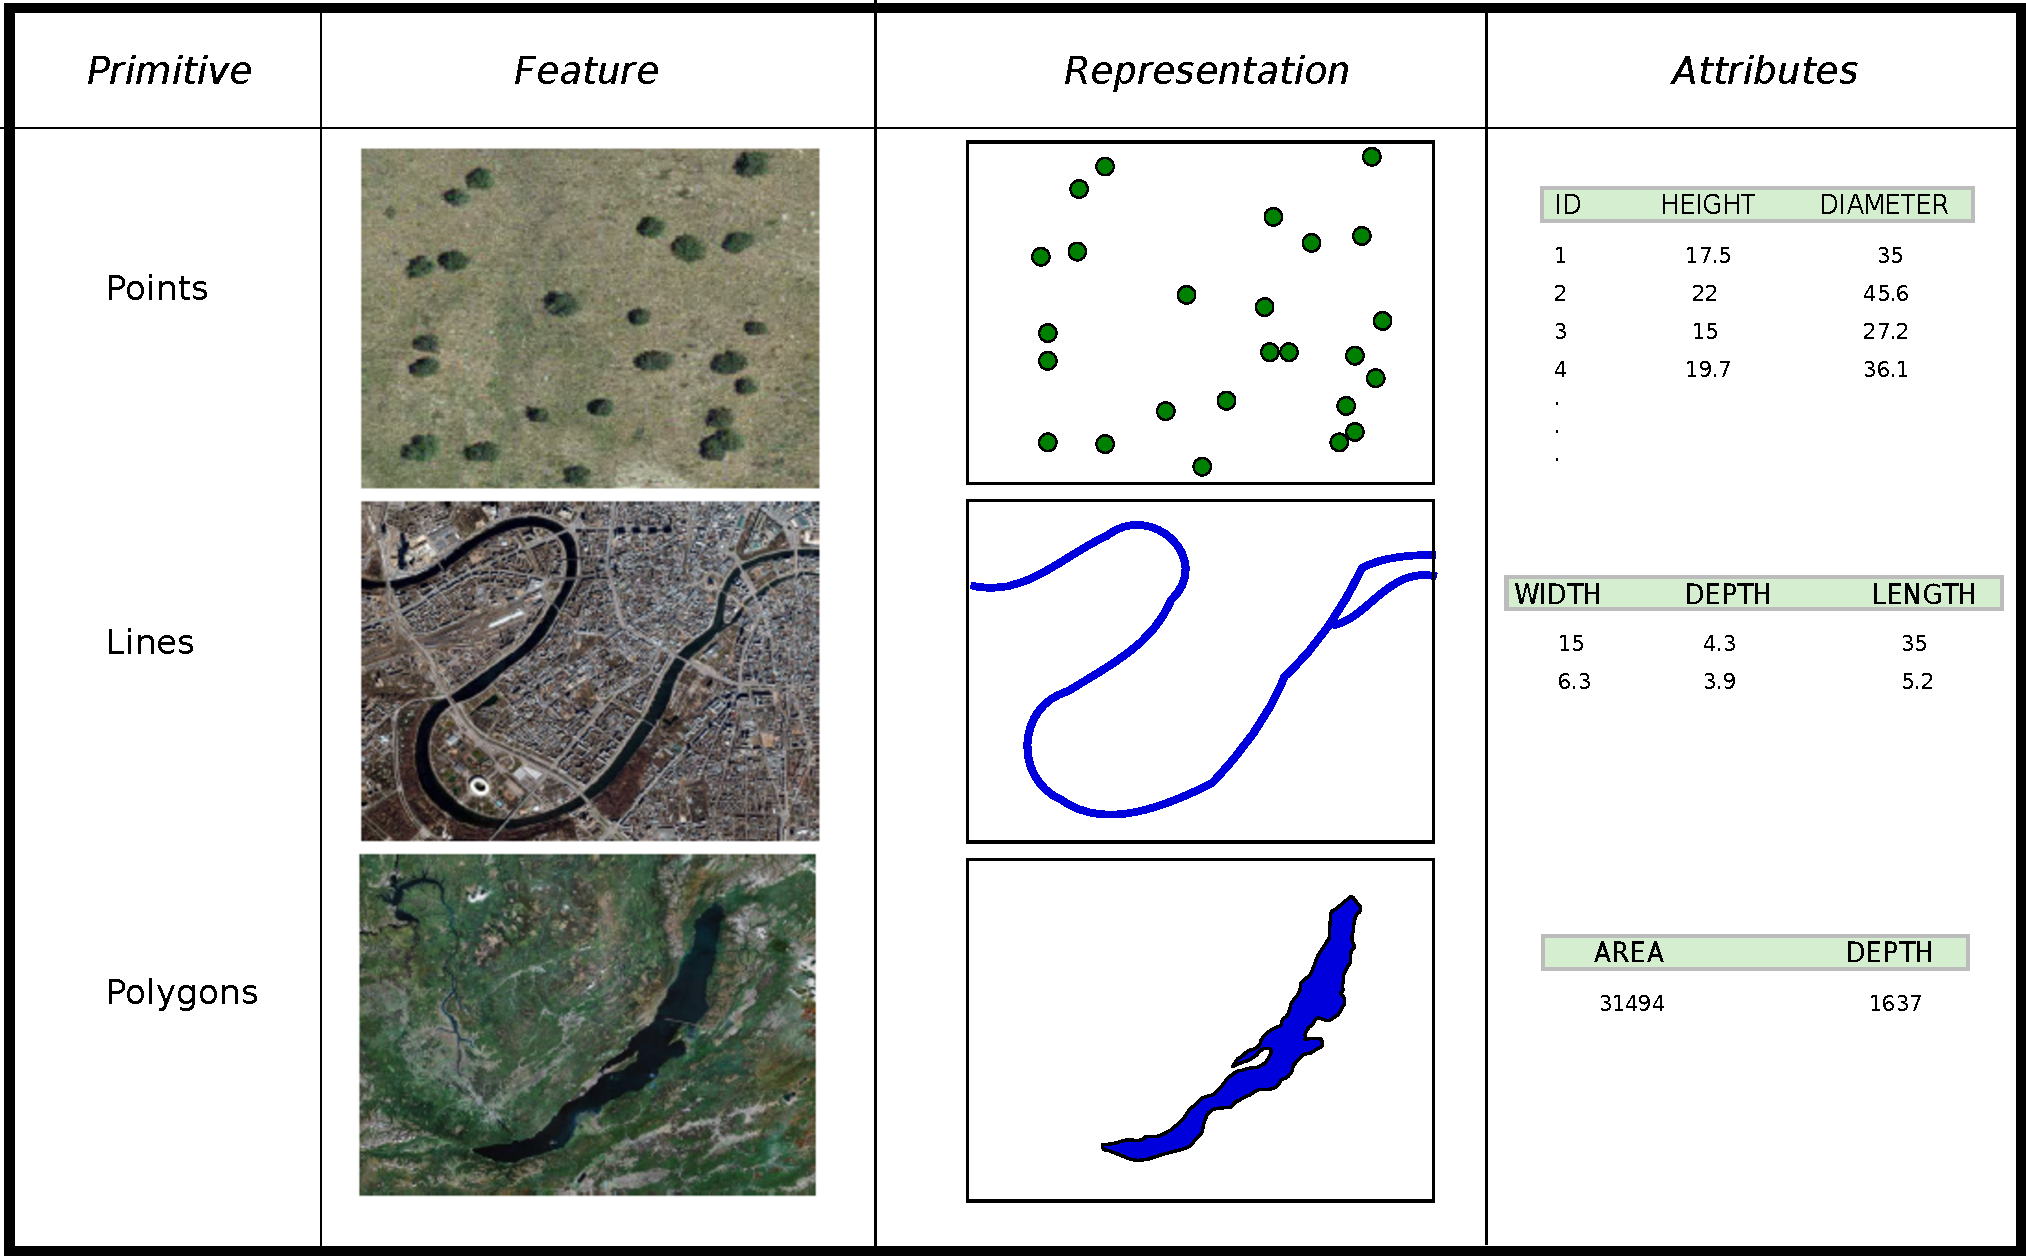
\includegraphics[width=\textwidth]{Data/Primitives.pdf}
\caption{\small Geometric primitives in the vector representation model and some examples of each of them and their associated attributes}
\label{Fig:Primitives} 
\end{figure}

Using points, lines and polygons, geographical space can be modeled by associating values to these primitives. A feature can have \textbf{multiple primitives}. For instance, in a layer that contains countries, a country such as the United States will require several polygons (continental US, Alaska, Hawaii islands, etc.). All those polygons form a single feature, since all of them belong to the same country and will share the same associated values.

A layer can contain features with primitives of different types, but usually it is restricted to just one single type. It is common to speak of a ``points layer'' or a ``polygons layer'' to indicate that. 

Elements can be represented using different types of primitives. For instance, a city can be represented as a single point or as a polygon with its perimeter. Using one or another geometry should depend on the type of phenomenon that we want to model or the level of detail that is needed, among other factors.

The thematic component in the vector model is defined using \textbf{attributes}. A layer usually contains multiple attributes. Attributes are associated to features, can have information of all types, and they are more versatile than the values associated to raster layers, which, as it was mentioned, normally contain just numerical values. Due to its particular structure (a set of attributes associated to a feature), the thematic component in the vector model can be represented as a table and stored in a \textbf{database} (we will see more about this in the chapter devoted to databases). Also, it can be be analyzed independently of the spatial component.

A particular element of the vector representation model is \textbf{topology}. A vector layer is said to contain topology if it contains the spatial relations between its features. Topology is required for certain analysis, and changes the way some operations, such as geometry editing, work in a GIS.

\begin{figure}[!hbt]   
\centering
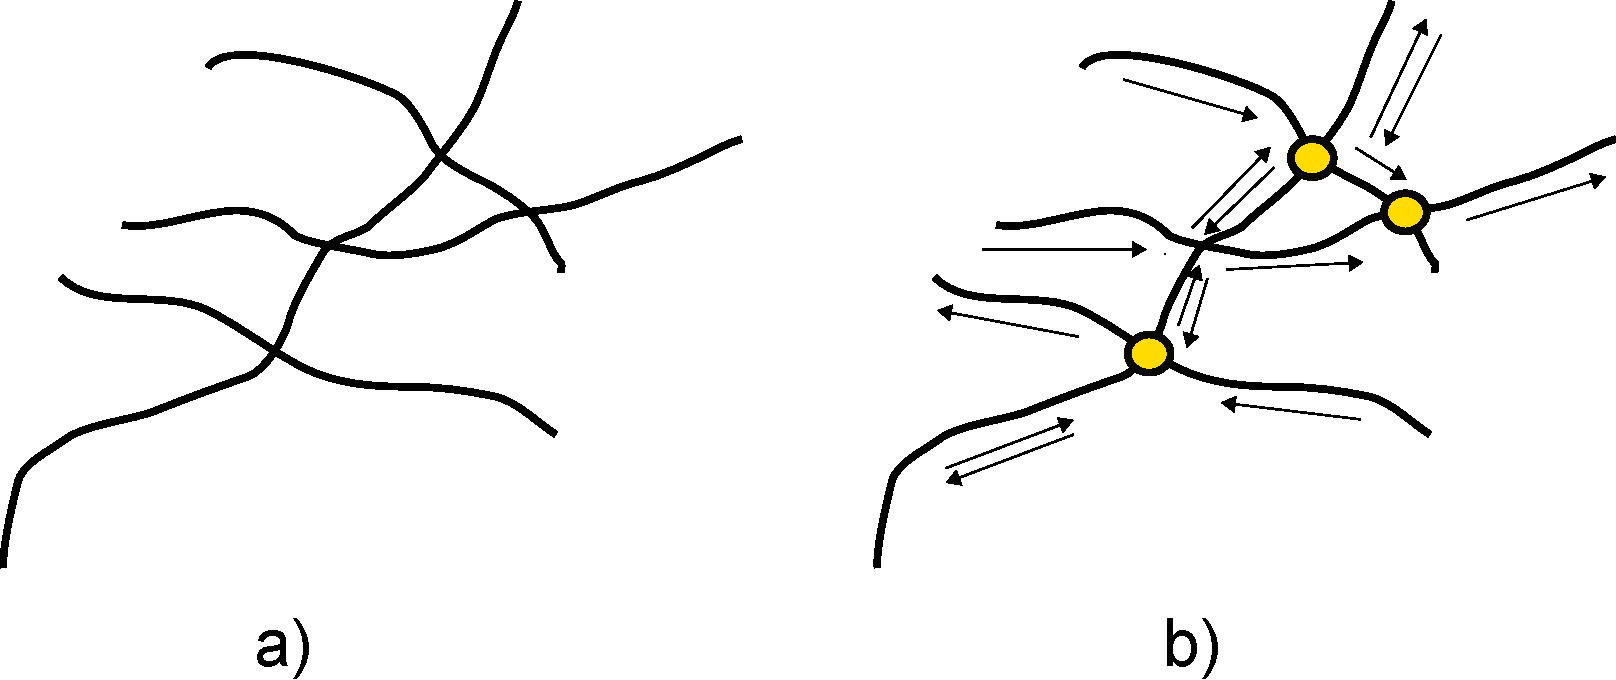
\includegraphics[width=.8\columnwidth]{Data/Topology_roads.pdf}
\caption{\small A roads layer without topology (a) and with topology (b). Circles in this last case indicate connections between roads.}
\label{Fig:Topology_roads} 
\end{figure}

Although most vector layer operations can be performed without topology, some of them such as \textbf{network analysis} are not possible without it. If we think about a roads layer, if it just contains lines representing roads but no information about how they are connected, there is no way of constructing the network from them. The points where lines intersect might be crossings or roundabouts (so it is possible to move from one road to another), but they might also be points without connection between the roads (one passing above the other). Without knowing that, we are missing information, and the network analysis cannot be performed. (Figure \ref{Fig:Topology_roads})

Line data without topology is popularly know as \emph{spaghetti} data.


\subsection{Raster \emph{vs} vector}


Both the raster and vector representation models can be used to store \textbf{any geographical information}. Figure \ref{Fig:Representation_models} contains an example of that, and it shows a roads layer represented using both models. 

We mentioned DEMs as a typical case of raster layers. Representing elevation as a raster layer has many advantages, especially for performing analysis, but it is not the only option. We can have a vector layer with points (that will be the case if the elevation data comes for a topographic survey), or a lines layer with contour lines (which is the most common way of representing elevation in a traditional map).

\begin{figure}[!hbt]   
\centering
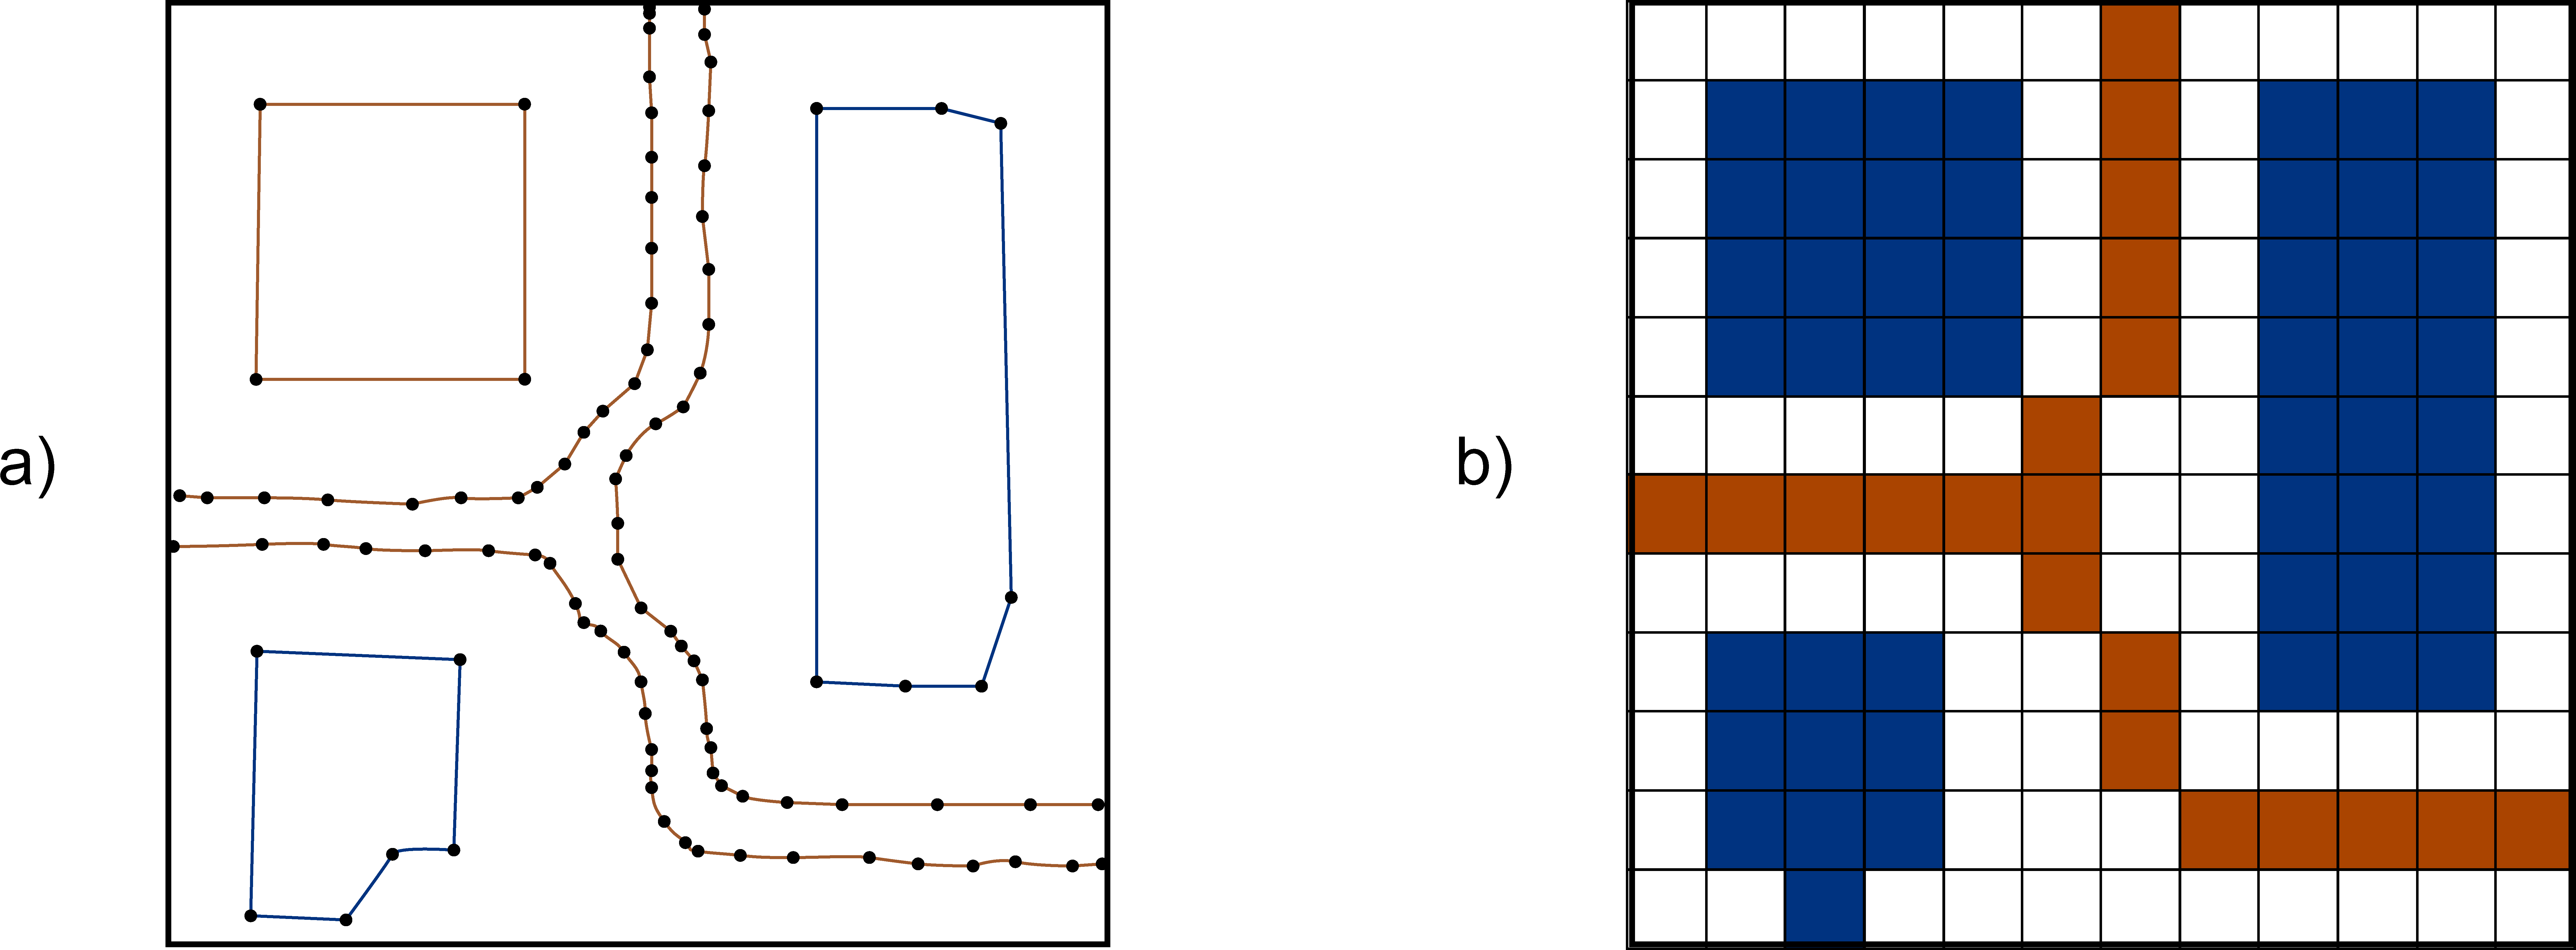
\includegraphics[width=\textwidth]{Data/Representation_models.pdf}
\caption{\small Comparison between vector (a) and raster (b) representation models.}
\label{Fig:Representation_models} 
\end{figure}

It is clear that both models have many differences, and each of them has it pros and cons. The following are some ideas to compare between them.


\begin{itemize}
\item \textbf{Approach}. Raster model focuses on the properties of the space that is represented (\emph{what} and \emph{how}), while the vector model focuses on the location of that property (\emph{where}).
 \item \textbf{Accuracy}. Raster model has its precision limited by the cell size. While this can be as small as we want, that would result in very large amounts of data. Features smaller than that size cannot be represented, and it is assumed that there is no variability within a cell.

 Also, shapes are limited to straight angles, since the base unit for the raster grid, as we have seen, it is a square or rectangle (Figure \ref{Fig:Raster_accuracy}

\begin{figure}[!hbt]   
\centering
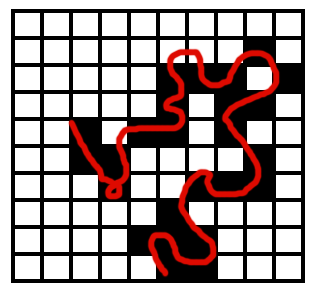
\includegraphics[width=.4\columnwidth]{Data/Raster_accuracy.png}
\caption{\small Limitations of the raster representation model. Since the space is divided in square units, elements such as curves cannot be faithfully represented.}
\label{Fig:Raster_accuracy} 
\end{figure}

\item \textbf{Complexity}. Analysis algorithms, specially those in which several layers are used and combined, are usually simpler and easier to implement with raster layers, mainly due to their regularity and systematicity. Working with vector layer, which do not have any regularity, tends to be more complex from the algorithmic point of view.
\end{itemize}

Overall, there is no representation model that is better than the other. Depending on the case, one will be more suitable than the other. The following factors should be considered when evaluating the suitability of these models to a particular circumstance:

\begin{itemize}
 \item \textbf{Type of variable or phenomenon to represent}. In general, it is better to use raster layers for \textbf{continuous} variables such as elevation, in order to make it easier to perform analysis based on them. \textbf{Discrete} variables, on the other hand, are better represented using a vector approach.
\item \textbf{Layer purpose}. It is important to know how we plan to use a layer, to decide the representation model that might better suit our case. For instance, if we have elevation data and we plan to perform analysis, it will be better to have a raster DEM, since most algorithms require the elevation data to be raster layer. However, if we want to use that elevation data just for visualization and combine it with other layers to create a map, it might be better to have a vector layer with contour lines, since those will be a better cartographic solution and will interfere less with the remaining variables. 
\item \textbf{Context}. The context might make it better (or even mandatory) to work with a given representation model. For instance, if we are working with images and we plan to do some analysis with other layers as well, those should be raster layers, since images, as we have seen, are always raster layers.
\end{itemize}

There are algorithms that allow \textbf{converting between the raster and vector representation models}, so if we have our data in one of them, we can obtain a new layer that uses the other model and might be more suitable for our work.

\pagestyle{empty}